\chapter{Proponowany model zjawiska}
\section{Koncepcja ’Social force’ i cele modelu}
\hspace{4ex}Wiele osób ma poczucie, że ludzkie zachowania są {\it chaotyczne} lub przynajmniej bardzo nieregularne i nieprzewidywalne. W rzeczywistości, szczególnie w dużych zbiorowiskach, ludzkie zachowanie można opisać jako model matematyczny, a w związku z tym da się przewidzieć zachowanie ludzi.
\par \medskip
Sugeruje się, że ruch pieszych można opisać tak, jak gdyby podlegał 'Social Force'. Te siły nie są bezpośrednio wywierane przez środowisko zewnętrze pieszego, ale odzwierciedlają one wewnętrzne motywacje pieszego do wykonywania określonych czynności jako odpowiedź na interakcje ze środowiskiem zewnętrznym. W prezentowanym modelu zachowań pieszych zasadnicze znaczenie ma kilka sił. Po pierwsze, konstrukcja opisująca siłę związaną z oczywistym dążeniem pieszego do wyjścia czy przejścia. Po drugie, konstrukcja odzwierciedlająca wpływ innych pieszych, między innymi związana z zachowaniem pewnej odległości pomiędzy pieszymi, tzw. strefy komfortu, a także umożliwiającej pieszemu wykonanie kolejnego kroku. Po trzecie, konstrukcja będąca odzwierciedleniem wpływu wszelkiego rodzaju przeszkód np. ścian. Często dodaje się również składową odzwierciedlającą siłę przykuwania uwagi pieszego do czegoś interesującego, a także siłę odzwierciedlającą to, że często piesi poruszają się w grupach znajomych.

Komputerowe symulacje ruchu oddziałujących na siebie pieszych pokazują, że model 'Social force' jest bardzo realistycznie.
\section{Formułowanie modelu 'Social force'}
\subsection{Ogólne równanie}
\hspace{4ex}Zgodnie z koncepcją 'Social force' przez {\it Helbing \& Molnar 1995} możemy uznać, że ruch pieszego można opisać za pomocą trzech różnych składowych tak, że 
$$f_{i}^{o}$$  \centerline{wewnętrzne zachowanie, odzwierciedlające motywację pieszego} \centerline{do poruszania się w określonym kierunku z określoną prędkością (wkierunku wyjścia)} 
$$f_{i}^{wall}$$ \centerline{wpływ ścian korytarza na tego pieszego}
$$f_{ij}$$ \centerline{efekty oddziaływania pieszego j na pieszego i.}
\par \medskip W tym momencie, poznamy zmianą prędkości $v_{i}$ pieszego i teraz możemy sformułować całościowe równanie
$$
\frac{dv_{i}}{dt} = f_{i}^{o} + f_{i}^{wall} + f_{ij}
$$
\subsection{Składowe siły 'Social Force'}
\hspace{4ex}Łatwo zauważamy, że wykorzystujemy dane eksperymentalne do sprawdzenia poprawności powyższego równania i określenia najważniejszej funkcji interakcji $f_{ij}$. Przejdźmy przez wszystkie komponenty.
\subsubsection{Zachowanie pojedynczego pieszego}
\hspace{4ex}Zgodnie z koncepcją 'Social force' przez {\it Helbing \& Molnar 1995} otrzymujemy równanie dla wewnętrznego przyspieszenia $\vec{f_i^o}$:
$$\vec{f_{i}^{o}} = \frac{v_i^oe_i^o-v_{i}(t)}{\tau}$$

Gdy (wszystkie poniższe stałe pochodzą z książki {\it Helbing  1995}),\\ \centerline{$v_i^o = 1.29 \pm 0.19(ms^{-1})$ : pożądane prędkości}
\centerline{$v_i(t) (ms^{-1})$ : aktualna prędkość}
\centerline{$\tau = 0.54 \pm 0.05(s)$: czas relaksacji}
\centerline{$e_i^o$: pożądany kierunek ruchu}
\subsubsection{Wpływ ścian na tym pieszym}
\hspace{4ex}Zgodnie z wcześniejszymi ustaleniami przez {\it Johansson et al. 2007} takie efekty ścian korytarzy na tym pieszym można opisać za pomocą równania:
$$
f_i^{wall}(d_w) = ae^{\frac{-d_w}{b}}
$$
Gdy, \\
\centerline{$d_w (m)$ : odległość prostopadła od pieszego do ściany}
\centerline{$a = 3$ i $b = 0.1$ : parametry odpowiadające siłom odpychania tego samego rzędu}
\subsubsection{Interakcje międzyludzkie}
\hspace{4ex}Również zgodnie z poprzednimi badaniami {\it Johansson et al. 2007}, wiemy, że interakcje międzyludzkie $f_{ij}$ mogą być definiowane jako funkcja odległości i kąta pomiędzy prostymi reprezentującymi kierunki ruchu pieszego i i j. podejścia okazują się jasne i uzasadnione $f_{ij}(d,\theta)$ Daje nam to równanie
$$
f_{ij}(d,\theta) = -Ae^{\frac{-d}{B}}(e^{-(n'B\theta)^2}t + e^{-(nB\theta)^2}n)
$$
Gdy,\\
\centerline{$n_{ij}$ : zmiany kierunkowe jako wektor jednostkowy w lewą stronę $\vec{t_{ij}}$}
\centerline{$d(m)$ : odległość między dwoma pieszymi $i$'em i $j$'em}
\centerline{$\theta(rad)$ : kąt między kierunkiem interakcji a wektorem skierowanym od pieszego $i$ do $j$}
\centerline{$A = 4.5 \pm 0.3$}
\centerline{$n' = 2.0 \pm 0.1$}
\centerline{$n = 3.0 \pm 0.7$}
\centerline{$t_{ij} = \frac{\vec{D_{ij}}}{\Vert \vec{D_{ij}} \Vert}$ : kierunek interakcji}\\
\par
Przyjrzyjmy się bliżej parametrowi B: jest zwiększany w kierunku interakcji przez duże prędkości względne i jest zmniejszone, gdy następuje odpychanie w kierunku boków. B zależy więc od:
$$
B = \gamma \Vert D \Vert
$$
Gdy,\\
\centerline{$\gamma = 0.35 \pm 0.01$ : parametr równania}
I mamy \\ \centerline{$\vec{D_{ij}} = \lambda(\vec{v_i} - \vec{v_j}) + \vec{e_{ij}}$}
\centerline{$\lambda = 2.0 \pm 0.2$ : względne znaczenie dwóch kierunków}
\centerline{$\vec{e_{ij}} = \frac{\vec{x_j}-\vec{x_i}}{\Vert \vec{x_j} - \vec{x_i} \Vert}$ : kierunek, w którym porusza się pieszy $j$}

Wykorzystaliśmy początkowo stałe wyznaczone w pracy Helbinga z 2009 roku, później poddaliśmy je kalibracji na własnym modelu.

\section{Diagramy}
\subsection{Diagramy cykli działań}
\subsubsection{Agent}
Diagram cykli działań dla jedno agenta
\begin{figure}[ht]
\centering
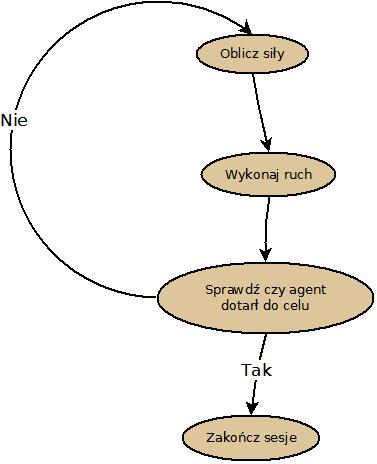
\includegraphics[scale=0.5]{DiagramAgent}
\caption{Diagramy działania dla jednego agenta}
\end{figure}

\subsubsection{Symulacja}
Diagram cykli działań symulacji ruchu pieszych
\begin{figure}[ht]
\centering
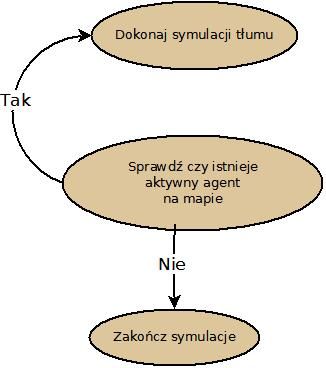
\includegraphics[scale=0.5]{DiagramAgenty}
\caption{Diagramy działania symulacji}
\end{figure}

\subsection{Diagramy przypadków użycia}

\subsubsection{Przypadki użycia systemu symulacji}
\begin{figure}[ht]
\centering
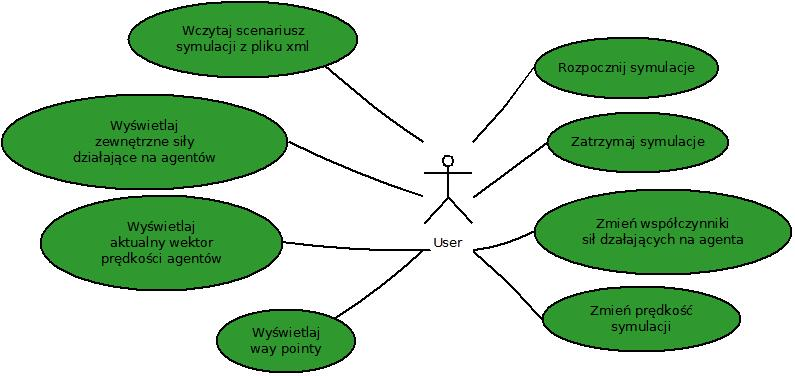
\includegraphics[scale=0.7]{UseCaseCalculate}
\caption{Diagramy przypadków użycia systemu symulacji}
\end{figure}


